%%%%%%%%%%%%%%%%%%%%%%%%%%%%%%%%%%%%%%%%%
% Beamer Presentation
% LaTeX Template
% Version 1.0 (10/11/12)
%
% This template has been downloaded from:
% http://www.LaTeXTemplates.com
%
% License:
% CC BY-NC-SA 3.0 (http://creativecommons.org/licenses/by-nc-sa/3.0/)
%
%%%%%%%%%%%%%%%%%%%%%%%%%%%%%%%%%%%%%%%%%

%----------------------------------------------------------------------------------------
%	PACKAGES AND THEMES
%----------------------------------------------------------------------------------------

\documentclass[UTF8]{ctexbeamer}

\usepackage{hyperref}
\hypersetup{
  colorlinks=true,
  linkcolor=red,
  anchorcolor=blue,
  citecolor=green
}

\mode<presentation> {

% The Beamer class comes with a number of default slide themes
% which change the colors and layouts of slides. Below this is a list
% of all the themes, uncomment each in turn to see what they look like.

%\usetheme{default}
%\usetheme{AnnArbor}
%\usetheme{Antibes}
%\usetheme{Bergen}
%\usetheme{Berkeley}
%\usetheme{Berlin}
%\usetheme{Boadilla}
%\usetheme{CambridgeUS}
%\usetheme{Copenhagen}
%\usetheme{Darmstadt}
%\usetheme{Dresden}
%\usetheme{Frankfurt}
%\usetheme{Goettingen}
%\usetheme{Hannover}
%\usetheme{Ilmenau}
%\usetheme{JuanLesPins}
%\usetheme{Luebeck}
\usetheme{Madrid}
%\usetheme{Malmoe}
%\usetheme{Marburg}
%\usetheme{Montpellier}
%\usetheme{PaloAlto}
%\usetheme{Pittsburgh}
%\usetheme{Rochester}
%\usetheme{Singapore}
%\usetheme{Szeged}
%\usetheme{Warsaw}

% As well as themes, the Beamer class has a number of color themes
% for any slide theme. Uncomment each of these in turn to see how it
% changes the colors of your current slide theme.

%\usecolortheme{albatross}
%\usecolortheme{beaver}
%\usecolortheme{beetle}
%\usecolortheme{crane}
%\usecolortheme{dolphin}
%\usecolortheme{dove}
%\usecolortheme{fly}
%\usecolortheme{lily}
%\usecolortheme{orchid}
%\usecolortheme{rose}
%\usecolortheme{seagull}
%\usecolortheme{seahorse}
%\usecolortheme{whale}
%\usecolortheme{wolverine}

%\setbeamertemplate{footline} % To remove the footer line in all slides uncomment this line
%\setbeamertemplate{footline}[page number] % To replace the footer line in all slides with a simple slide count uncomment this line

%\setbeamertemplate{navigation symbols}{} % To remove the navigation symbols from the bottom of all slides uncomment this line
}

\usepackage{graphicx} % Allows including images
\graphicspath{{./figs/}}
\usepackage{booktabs} % Allows the use of \toprule, \midrule and \bottomrule in tables

% Fonts
% \usepackage{libertine}
% \setmonofont{Courier}
\setCJKsansfont[ItalicFont=Noto Serif CJK SC Black, BoldFont=Noto Sans CJK SC Black]{Noto Sans CJK SC}

%----------------------------------------------------------------------------------------
%	TITLE PAGE
%----------------------------------------------------------------------------------------

\title[第1讲]{第1讲 :操作系统概述} % The short title appears at the bottom of every slide, the full title is only on the title page

\author{向勇、陈渝} % Your name
\institute[清华大学] % Your institution as it will appear on the bottom of every slide, may be shorthand to save space
{
清华大学计算机系 \\ % Your institution for the title page
\medskip
\textit{xyong,yuchen@tsinghua.edu.cn} % Your email address
}
\date{\today} % Date, can be changed to a custom date

\begin{document}

\begin{frame}
\titlepage % Print the title page as the first slide
\end{frame}

\begin{frame}
\frametitle{提纲} % Table of contents slide, comment this block out to remove it
\tableofcontents % Throughout your presentation, if you choose to use \section{} and \subsection{} commands, these will automatically be printed on this slide as an overview of your presentation
\end{frame}

%----------------------------------------------------------------------------------------
%	PRESENTATION SLIDES
%----------------------------------------------------------------------------------------

%------------------------------------------------
\section{第八节:OS实验概述} % Sections can be created in order to organize your presentation into discrete blocks, all sections and subsections are automatically printed in the table of contents as an overview of the talk
%------------------------------------------------
\subsection{单用户系统}
\subsection{批处理系统}
\subsection{多道程序系统}
\subsection{分时系统}
\subsection{个人计算机}
\subsection{分布式计算}

\begin{frame}

\frametitle{OS实验概述}

\begin{itemize}
\item 设计思路
    \begin{itemize}
    \item 采用小巧全面的操作系统ucore并进行改进,需要覆盖操作系统的关键点,为此增加:
    \begin{itemize}
        \item 外设:I/O管理/中断管理
        \item 内存:虚存管理/页表/缺页处理/页替换算法
        \item CPU:进程管理/调度器算法
        \item 并发:信号量实现和同步互斥应用
        \item 存储:文件系统+磁盘驱动
    \end{itemize}
    \item 完整代码量控制在10000行以内
    \item 提供实验讲义和源码分析文档
    \end{itemize}
\end{itemize}

\end{frame}


\begin{frame}
	
	\frametitle{OS实验内容}

	\begin{columns}
    \begin{column}{.35\linewidth}
    OS实验内容
	\begin{enumerate}
	    \item OS启动/中断/异常
		\item 物理内存管理
		\item 虚拟内存管理	
		\item 内核模式线程管理
		\item 用户模式进程管理
		\item 处理器调度
		\item 多处理与同步互斥
		\item 文件系统
	\end{enumerate}
	\end{column}
	
	\begin{column}{.7\linewidth}
	\begin{figure}
		\centering
		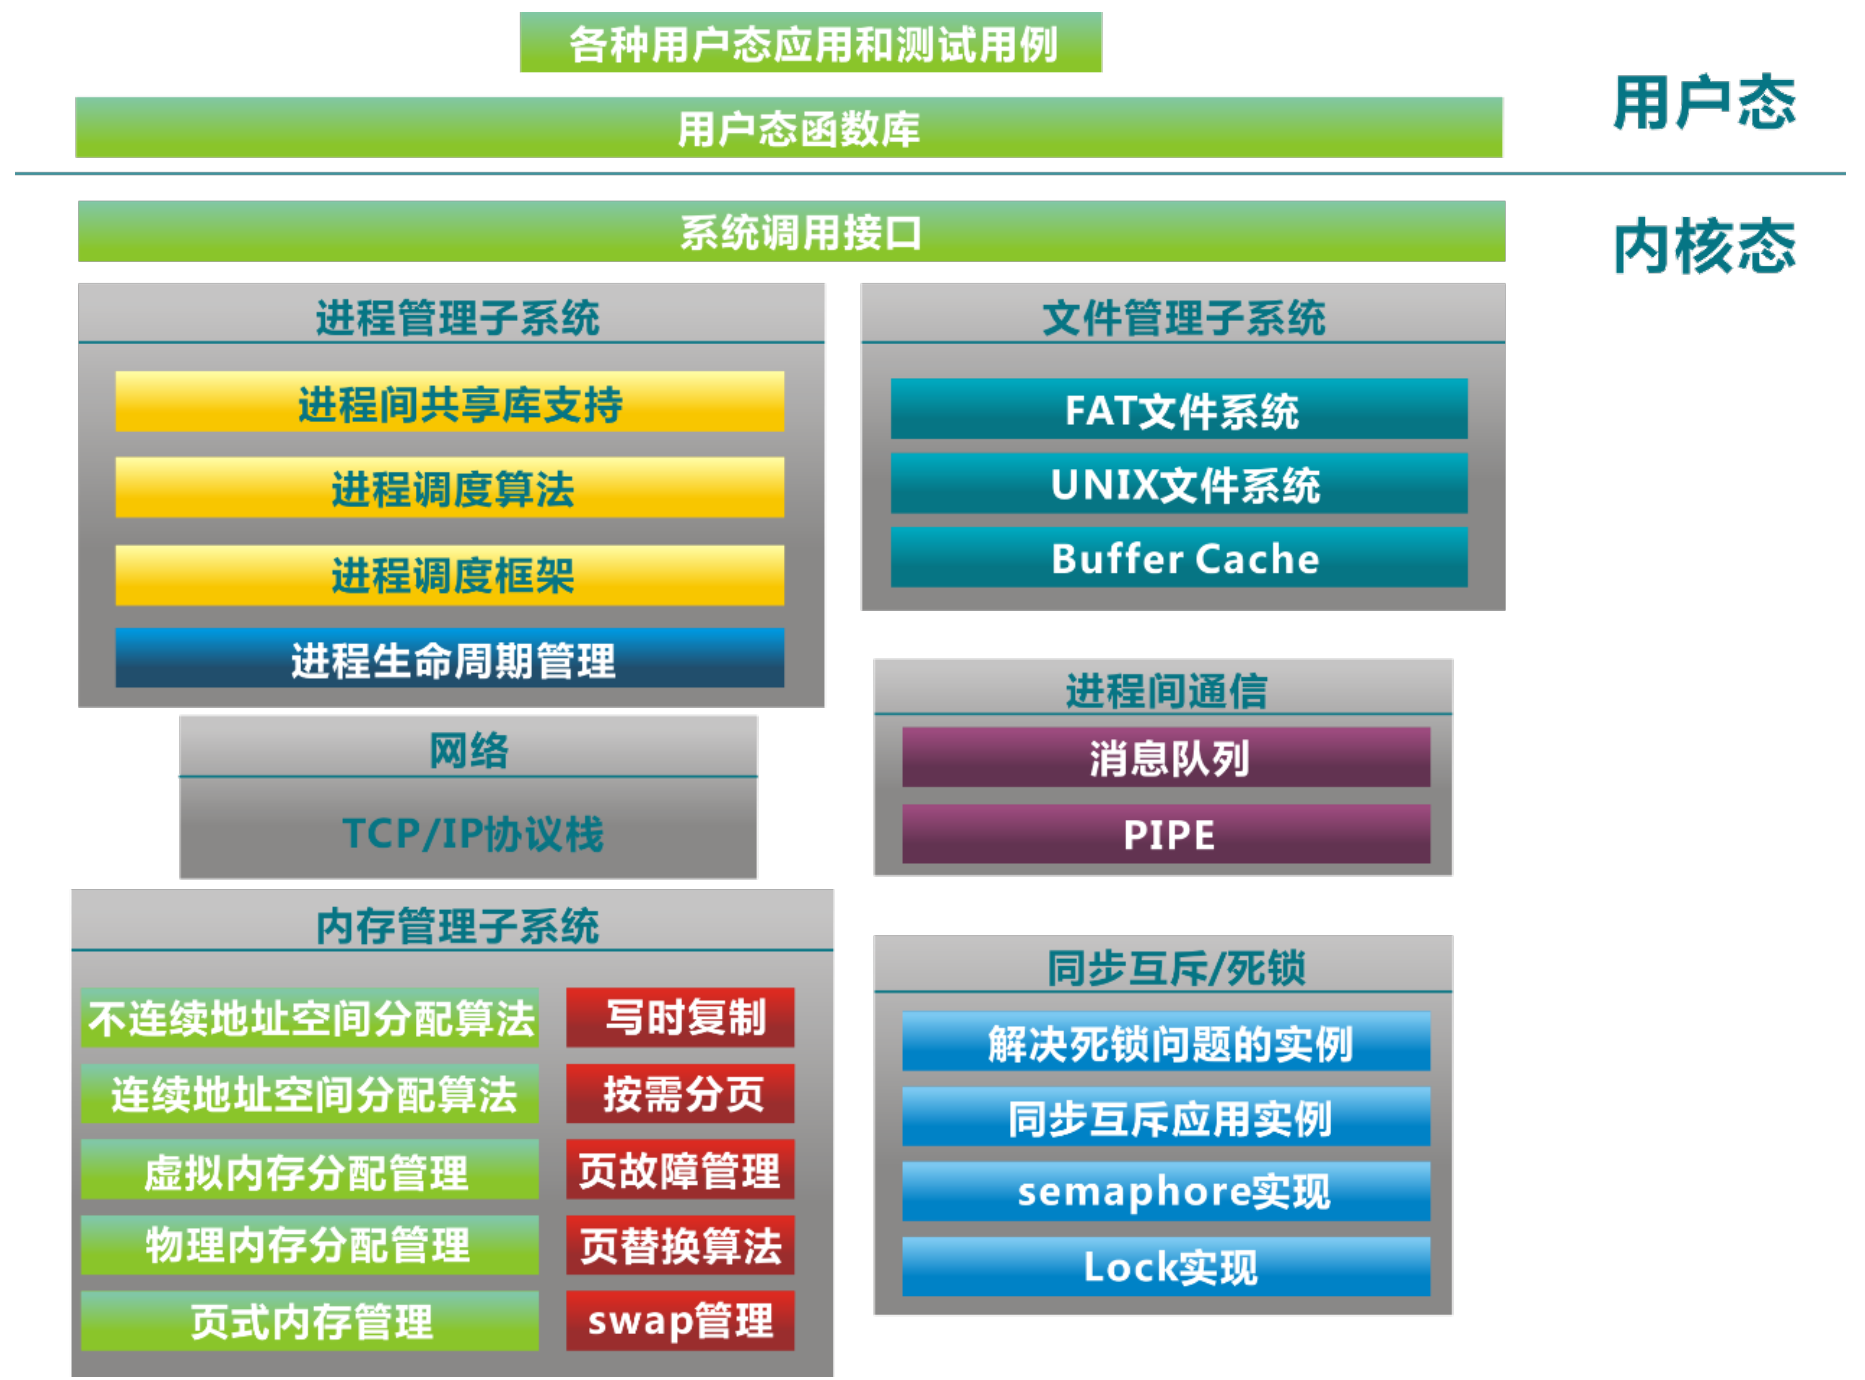
\includegraphics[width=1.0\linewidth]{oslab-overview}
		\caption{OS实验框架}
	\end{figure}
	\end{column}
	\end{columns}
\end{frame}


\begin{frame}
\frametitle{OS实验内容}
\framesubtitle{lab1}
	
\end{frame}


\begin{frame}
\frametitle{OS实验内容}
\framesubtitle{lab2}
	
\end{frame}

\begin{frame}
\frametitle{OS实验内容}
\framesubtitle{lab3}
	
\end{frame}

\begin{frame}
\frametitle{OS实验内容}
\framesubtitle{lab4}
	
\end{frame}


\begin{frame}
\frametitle{OS实验内容}
\framesubtitle{lab5}
	
\end{frame}

\begin{frame}
\frametitle{OS实验内容}
\framesubtitle{lab6}
	
\end{frame}


\begin{frame}
\frametitle{OS实验内容}
\framesubtitle{lab7}
	
\end{frame}


\begin{frame}
\frametitle{OS实验内容}
\framesubtitle{lab8}
	
\end{frame}

%----------------------------------------------------------------------------------------

\end{document}
